\section{Unique Approaches}

To apply perceptron q-learning to Super Smash Brothers Melee, outside the box techniques were required to deal with discontinuities in optimal behavior, "action-lockout", large state-evolution time scales, and fringe cases of large delays between an action its direct result.

\subsection{Discontinuity in Optimal Behavior}
In Super Smash Brothers Melee, the optimal action largely depends on the current state. An issue arises in global-approximation techniques when nearby states should have dissimilar optimal actions. An example of this is the case of an agent standing on the edge of the stage, in which its goal is to deal damage to the opponent, and an agent being slightly off of the stage (about to fall to its death unless some preventative action is taken), in which it should make an effort to navigate back to the stage and avoid dying. This problem was initially identified when the agent was frequently observed issuing attacking commands while falling to its death near the edge of the stage. We believe this was due to the agent extrapolating from the nearby extremely favorable state action of standing on the edge of the stage while hitting its opponent. This combination is favorable due to the opportunity to knock the opponent off the stage, scoring a kill.

To prevent generalization from nearby but dissimilar states, we discretized the environment into an additional three super-states: off the stage to the left, on the stage, and off the stage to the right. These super-states represent different situations in which the optimal behavior of the agent should be completely discrete from a nearby state that is in a different super-state. As discussed in the applications section, a padded beta vector is created $\beta_{p} = [\beta,~0_{|\beta|},~0_{|\beta|}]$, where $0_{|\beta|}$ denotes a vector of $|\beta|$ zeros. The base $\beta$ function is then inserted to the appropriate super-index of the padded basis function. The result is a training of different perceptron weights in different super-states for each map partition, and a prevention of generalizing between states that should not be generalized between. 

This change during development vastly improved the agents ability to survive being knocked off of the stage. The agent now jumps back towards the stage in an often successful effort to survive (and avoid penalties for dying). 

\subsection{Action Lockout}
Another issue to be addressed was the impact of ”action-lockout”, in which an action taken by the agent may have no impact on its current in game movements due to previous actions taken. An example of this is when the agent selects an action with a long wind-up animation that cannot be canceled by other actions. To address this, actions that are taken during an "action-lockout" are ignored during the training process of the basis function weights. 

\subsection{State Evolution}
In the game environment, the state evolves relatively slowly from each action taken. The game runs at 60hz and it is possible to send a unique input on every frame, however it is clear that the game was not designed to be played this way. The problem with this is the lead time between an action taken, the windup animation from the resulting action, and the change in the current state space as a result of this action. To deal with this, the agent was limited to observing and acting five times a second, or once every twelve frames. When an action is selected, the agent inputs that controller inputs and holds the inputs until a new action is selected. This choice was made as it mimics a humans capabilities of action inputs and better meshes with the intended gameplay.

While performing batch learning, this is taken into account. In the weight update process, $\theta_a\beta(s)$ of the last action take is used for each update, while the state $s'$ is taken as usual. The rewards are computed at each state step and assigned back to the last action taken. The result is that the original state action pair is rewarded for the state evolution that occurs, rather than rewarding the action at intermediate states of the evolution. 

\begin{figure}[!htb]
	\centering
	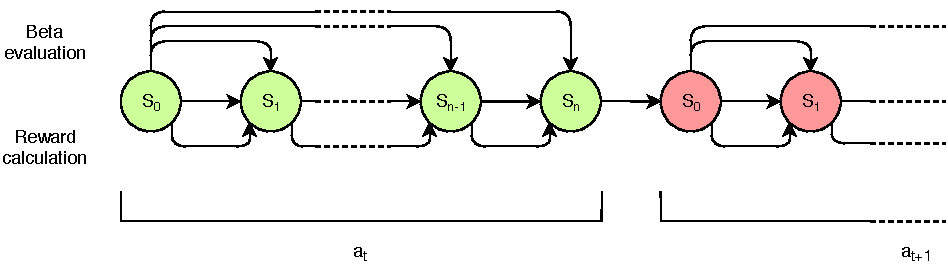
\includegraphics[width=120mm]{stateevolution.pdf}
	\caption{State evolution}
\end{figure}

\subsection{Action Impact Delay}

Dealing with rewards for kills and deaths was not straight forward due to the large lag between an action that resulted in one of these events and the event occurring. To assign rewards to killing the opponent, the last action the agent took that dealt damage is recorded as a "last damaging action". When the opponent dies, a large reward is assigned to this "last damaging action". This is necessary to avoid assigning large rewards to actions that do not cause the opponent to die, and is equivalent to knowing immediately after the action is taken if it will result in the death of the opponent despite the game not providing this information.





